\chapter{Numerical Results}
\label{chap:results}

Five test problems have been developed for evaluating the nonlinear solver, the operator based scaling, the convergence metric, the domain decomposition algorithm, and the selective nonlinear refinement.
Two geometrically simple problems were developed to evaluate the nonlinear solver, the operator based scale factor, and the temporal convergence metric.
One problem with extensive geometric complexity was used to evaluate the domain decomposition algorithm.
Two problems were developed to test the selective nonlinear refinement.
The goal of the tests, the methods used, and the models will be discussed in each section.

\section{Single Phase Flow and Flashing Problems}
\label{sect:single_phase_and_flashing}

Two test problems were developed to illustrate the effectiveness of the nonlinear solver and the operator based scaling.
The two problems were set up so that the maximum allowable timestep was varied.
Each problem was run with the following maximum allowable timesteps: 1 [s], 0.1 [s], 0.01 [s], 0.001 [s], 0.0001 [s], and 0.00001 [s]. 
For the linear runs, the scaled residuals were evaluated after a single Newton step, $\vec{F}(\vec{x}^{1})$.
For the nonlinear runs, the scaled nonlinear residuals were evaluated at the end of the Newton-loop.
The nonlinear convergence criteria used in the nonlinear solver are described in \sect{sect:nlnCobraAlg}.
The temporal convergence metric was evaluated during post-processing.
In total, there were twenty-four simulations run.
The two different problems were each run at six different maximum timestep sizes on each of the two versions of \cobra{}.

\subsection{Model}
\label{subsect:single_model}
For both of the test problems, the same computational geometry was used;  \fig{fig:exp_geometry} represents the experimental geometry.
Each block represents a single continuity cell with a height of 4 [in].
The total height of the channel is 48 [in].
Each continuity cell has a cross-sectional area of 4 [in$^2$].
The red block at the top of the channel represents a boundary cell where the pressure and enthalpy are specified.
It represents an infinite reservoir filled with a fluid at a specified thermodynamic state.
The red triangle represents a specified flow at the bottom edge of the first continuity cell. 

\begin{figure}[h!t]
\centering
\tikzsetnextfilename{images/scaling_test_problem_geometry_pdf}
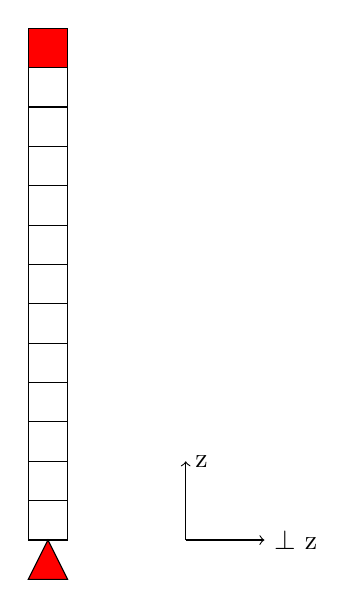
\begin{tikzpicture}
\foreach \x in {1,..., 12} \draw(0, 0.5*\x-0.5) rectangle +(.5,.5);
\filldraw[fill=red] (0, 6) rectangle +(.5,.5); 
\filldraw[fill=red] (0, -0.5) -- (0.25, 0) -- (0.5, -0.5) -- cycle;
\draw[->] (2,0) -- (2, 1) node[anchor=west] {z};
\draw[->] (2,0) -- (3, 0) node[anchor=west] {$\perp$ z};
\end{tikzpicture}
\caption{Geometry for test problems.}
\label{fig:exp_geometry}
\end{figure}

The two problems, while having the same geometry, are different in their dominant physics.
One problem was designed to simulate single-phase, single-field continuous liquid flow in a standpipe.
This problem will be referred to as the single-phase problem.
The second problem was designed such that high-pressure liquid flashes into steam as it enters a standpipe initially filled with saturated vapor at a much lower pressure, known hereafter as the flashing problem.

Table \ref{tab:ic} provides the initial conditions for the two problems.
The pressure, enthalpy, and volume-fractions for the different fields allow for a complete description of the continuity variables.
The initial velocities are set to zero.

\begin{table}[ht]
\centering
\pgfplotstabletypeset[fixed zerofill, col sep=comma,
	columns/problem/.style={column name=,string type, column type=l},
	columns/p/.style={ column name=Pressure,dec sep align, precision=1},
	columns/h/.style={ column name=Enthalpy,dec sep align, precision=1},
	columns/a_g/.style={ column name=$\alpha_g$, precision=1},
	columns/a_l/.style={ column name=$\alpha_l$, precision=1},
	columns/a_e/.style={ column name=$\alpha_e$, precision=1},
	every head row/.style={
		before row=\toprule,
		after row={& \multicolumn{2}{c}{$[\text{psia}]$} &\multicolumn{2}{c}{$[\frac{\text{BTU}}{\lbm{}}]$} &$[\text{-}]$ & $[\text{-}]$ & $[\text{-}]$\\ \midrule}},
	every last row/.style={
after row=\bottomrule}]{tables/data_ic_nln.tex}

\caption{Initial conditions for test problems.}
\label{tab:ic}
\end{table}

Each of the problems has a specified pressure-enthalpy boundary condition at the top of the stand pipe and a flow-enthalpy boundary condition at the inlet of the domain.
Table \ref{tab:bc_pe} contains the pressure, enthalpy, and composition of the pressure-enthalpy reservoir. 

\begin{table}[h!t]
\centering
\pgfplotstabletypeset[fixed zerofill, col sep=comma,
	columns/problem/.style={column name=,string type, column type=l},
	columns/p/.style={ column name=Pressure,dec sep align, precision=1},
	columns/h/.style={ column name=Enthalpy,dec sep align, precision=1},
	columns/a_g/.style={ column name=$\alpha_g$, precision=1},
	columns/a_l/.style={ column name=$\alpha_l$, precision=1},
	columns/a_e/.style={ column name=$\alpha_e$, precision=1},
	every head row/.style={
		before row=\toprule,
		after row={& \multicolumn{2}{c}{$[\text{psia}]$} &\multicolumn{2}{c}{$[\frac{\text{BTU}}{\lbm{}}]$} &$[\text{-}]$ & $[\text{-}]$ & $[\text{-}]$\\ \midrule}},
	every last row/.style={
after row=\bottomrule}]{tables/data_bc_outflow_nln.tex}

\caption{The pressure-enthalpy outlet boundary conditions for test problems.}
\label{tab:bc_pe}
\end{table}

The flow-enthalpy boundary condition describes the thermodynamic state of the in-flowing fluid and its flow rate.
Table \ref{tab:bc_fe} describes the inlet boundary condition for the two problems.

\begin{table}[ht]
\centering
\pgfplotstabletypeset[fixed zerofill, col sep=comma,
	columns/problem/.style={column name=,string type, column type=l},
	columns/p/.style={ column name=Pressure,dec sep align, precision=1},
	columns/h/.style={ column name=Enthalpy,dec sep align, precision=1},
	columns/a_g/.style={ column name=$\alpha_g$, precision=1},
	columns/a_l/.style={ column name=$\alpha_l$, precision=1},
	columns/a_e/.style={ column name=$\alpha_e$, precision=1},
	every head row/.style={
		before row=\toprule,
		after row={& \multicolumn{2}{c}{$[\text{psia}]$} &\multicolumn{2}{c}{$[\frac{\text{BTU}}{\lbm{}}]$} &$[\text{-}]$ & $[\text{-}]$ & $[\text{-}]$\\ \midrule}},
	every last row/.style={
after row=\bottomrule}]{tables/data_bc_inflow_nln.tex}

\caption{The flow-enthalpy inlet boundary conditions for test problems.}
\label{tab:bc_fe}
\end{table}

The specified mass flow, $\dot{m}(t)$, at the bottom of the channels is the same for both problems. 
This time-dependent function is given by \eqref{eqn:bc_time_func_single}.

\begin{equation}
\label{eqn:bc_time_func_single}
\dot{m}(t) = \left\{
\begin{array}{cclrcll}
 0.0           & [\frac{ \lbm{} }{\text{s}}] & , &                & t & \leq 1 & [\text{s}] \\
 0.5 ( t - 1)  & [\frac{ \lbm{} }{\text{s}}] & , & 1\; [\text{s}] < & t & \leq 2 & [\text{s}] \\
 0.5           & [\frac{ \lbm{} }{\text{s}}] & , &                & t & > 2    & [\text{s}]
\end{array}\right.
\end{equation}

Both problems adjust their initial pressure distribution to account for hydrostatic head, which is not specified in the input files.
The \cobra{} input files for both problems can be found in \app{app:input_decks}.

\subsection{Results}
\label{subsect:single_results}

The results from the simulation runs will now be analyzed to determine the impact of nonlinear convergence upon time-step size sensitivity.
The solutions produced by both solvers will be compared to determine the efficacy of the residual metric in determining the validity of the nonlinear solution.  

For the flashing problem, the parameter of interest for temporal convergence testing is $\alpha_g$ at 2 [in] from the inlet of the stand pipe.
\fig{fig:flashing_1em1} shows the gaseous volume fraction 2 [in] from the inlet of the stand pipe as a function of time for a \dtmax{} of 1.0E-1 [s] for both the linear and the nonlinear solvers.

\begin{figure}[h!tb]
\centering
\includegraphics[width=0.6\textwidth]{plots/flashing_1em1.eps}
\caption{Flashing solution at \dtmax{} = 1.0E-1 {[s]}}
\label{fig:flashing_1em1}
\end{figure}

\begin{figure}[h!tb]
\centering
\includegraphics[width=.6\textwidth]{plots/flashing_1em5.eps}
\caption{Flashing solution at \dtmax{} = 1.0E-5 {[s]}.}
\label{fig:flashing_1em5}
\end{figure}

Note that the nonlinearly resolved solution is qualitatively different than the linear single-shot solution, \fig{fig:flashing_1em1}.
Even as the \dtmax{} is reduced, this discrepancy does not disappear, \fig{fig:flashing_1em5}.
The two solutions do not converge to the same solution as the timestep size was reduced.
However, the solution to the flashing problem produced by the nonlinear solver, \fig{fig:nl_mode_flashing}, qualitatively varies less as the timestep size is reduced than that produced by the linear solver, \fig{fig:cobra_mode_flashing}.
However, both \fig{fig:cobra_mode_flashing} and \fig{fig:nl_mode_flashing} show that as the timestep size is reduced the two different solutions become more timestep size insensitive.

\begin{figure}[h!tb]
\centering
\includegraphics[width=.6\textwidth]{plots/lin_flashing_al_2in.eps}
\caption{Linear solver flashing solution.}
\label{fig:cobra_mode_flashing}
\end{figure}

\begin{figure}[h!bt]
\centering
\includegraphics[width=.6\textwidth]{plots/nln_flashing_al_2in.eps}
\caption{Nonlinear solver flashing solution.}
\label{fig:nl_mode_flashing}
\end{figure}

The two solvers, when applied to the same problem that contains highly nonlinear physics, produce two different timestep size invariant solutions.
These two solutions achieve qualitative timestep size invariance at different timestep sizes.
The parameter of interest in the solution produced by the nonlinear solver with a 1 [s] \dtmax{} is qualitatively close to that produced with a 0.1 [s] \dtmax{}, \fig{fig:nl_flashing_compare}.
The same level of qualitative timestep size invariance is achieved in the linear solver solutions between a \dtmax{} of 1.0E-3 [s] and 1.0E-4 [s], \fig{fig:cobra_flashing_compare}.

\begin{figure}[h!bt]
\centering
\includegraphics[width=.6\textwidth]{plots/nln_flashing_1em0_1em1.eps}
\caption{Nonlinear solver timestep size insensitive flashing solution.}
\label{fig:nl_flashing_compare}
\end{figure}

\begin{figure}[h!tb]
\centering
\includegraphics[width=.6\textwidth]{plots/lin_flashing_1em1_1em4.eps}
\caption{Linear solver timestep size insensitive flashing solution.}
\label{fig:cobra_flashing_compare}
\end{figure}

The timestep size insensitive solution produced by the nonlinear solver occurs at a maximum timestep size three orders of magnitude greater than that achieved by the linear solver in \cobra{}.
An examination of the nonlinear residual over the course of the transient provides insight into why this behavior is observed.
The scaled residual for the linear flashing problem indicates that, even for small timestep sizes, the solution obtained still does not satisfy the discrete nonlinear equations, \fig{fig:linear_flashing_residual}.
This is in contrast to the nonlinear flashing problem, which shows a lower residual over the course of the simulation, \fig{fig:nonlinear_flashing_residual}.

\begin{figure}[h!tb]
\centering
\includegraphics[width=0.6\textwidth]{plots/lin_flashing_res_compare.eps}
\caption{Residual of the flashing solution for the linear solver.}
\label{fig:linear_flashing_residual}
\end{figure}

\begin{figure}[h!tb]
\centering
\includegraphics[width=0.6\textwidth]{plots/nln_flashing_res_compare.eps}
\caption{Residual of the flashing solution for the nonlinear solver.}
\label{fig:nonlinear_flashing_residual}
\end{figure}

The reduction in the residual exhibited by the solution produced by the linear solver, \fig{fig:linear_flashing_residual}, shows that the reduction of the maximum allowable timestep size now serves two purposes.
The first is that as \dtmax{} is reduced the nonlinear physics are being better resolved; however, even for small \dtmax{}, the residuals are still large compared to those of the nonlinear solution, \fig{fig:nonlinear_flashing_residual}.
The second purpose in reducing \dtmax{} is to decrease the error due to the discrete approximation of the temporal integral of the governing equations.
While the reduction of the maximum timestep size in the linear solver serves the purpose of reducing the residual, the nonlinear solver performs this task naturally.
Therefore, in the nonlinear solver the reduction of the maximum timestep size primarily serves to reduce the error from the approximate discrete temporal integral.

\begin{figure}[h!tb]
\centering
\includegraphics[width=0.6\textwidth]{plots/single_1em0.eps}
\caption{Single-phase solution with \dtmax{} = 1.0 {[s]}.}
\label{fig:single_1em1}
\end{figure}

s\begin{figure}[h!tb]
\centering
\includegraphics[width=0.6\textwidth]{plots/single_1em5.eps}
\caption{Single-phase solution with \dtmax{} = 1.0E-5 {[s]}.}
\label{fig:single_1em5}
\end{figure}

The single-phase case was designed to test if the linear solver produced a simulation result that was equivalent to that produced by the nonlinear solver.
More specifically, it was designed to show that for problems where the physics of interest have relatively low nonlinearities, the linear solver provides as accurate a solution as the nonlinear solver.
\fig{fig:single_1em1} and \fig{fig:single_1em5} show the solution produced by both the nonlinear and linear solvers of \cobra{}.
Unlike the flashing problem, both solvers were able to solve the problem for all of the \dtmax{} specified.
The solutions produced by both solvers are qualitatively equivalent at \dtmax{} = 1.0 [s] and \dtmax{} = 1.0E-5 [s].
This indicates that the linear solver is adequate in regions where the solution is not highly nonlinear.

One way to quantify the difference between the solutions is by measuring the residual convergence metrics outlined in \sect{sect:temporal_convergence}.
These metrics provide a measure of how poorly the discrete nonlinear equations are being solved at every timestep in the transient.
The resolution of the residual allows for a solution that is less sensitive to timestep size selection than for a solution that does not resolve the residual.
The convergence metrics will be used to determine if a qualitative temporal-convergence determination can lead to the acceptance of a solution that is not nonlinearly converged.

For each of the test cases, the two different metrics were compared at the different \dtmax{}.
To examine efficacy of the the temporal convergence criteria, both the average and moment based temporal convergence criteria were evaluated for each of the twenty-three successful simulations.
The values of these metrics will be compared between different solvers for the same test problem. 

The two different nonlinear convergence metrics will now be examined for the flashing problem.
\tab{tab:flashing_criteria} shows both the average metric, $\tilde{R}$, and the moment based metric, $\tilde{R}_{\text{M}}$.

\begin{table}[h!t]
\centering
\pgfplotstabletypeset[sci zerofill,sci E, col sep=comma,
	columns/0/.style={ column name=\dtmax{}, precision=1},
	columns/1/.style={ column name=Linear, precision=3},
	columns/2/.style={ column name=Nonlinear, precision=3},
	columns/3/.style={ column name=Linear, precision=3},
	columns/4/.style={ column name=Nonlinear, precision=3},
	every head row/.style={
		before row={
			\toprule
			&\multicolumn{2}{c}{$\tilde{R}$} & \multicolumn{2}{c}{$\tilde{R}_{M}$}\\
		},
		after row=\midrule
	},
	every last row/.style={
after row=\bottomrule}]{tables/data_flashing_metric.tex}
\caption{Nonlinear convergence metrics for flashing problem.}
\label{tab:flashing_criteria}
\end{table}

\begin{table}[h!t]
\centering
\pgfplotstabletypeset[sci zerofill,sci E, col sep=comma,
	columns/0/.style={ column name=\dtmax{}, precision=1},
	columns/1/.style={ column name=Linear, precision=3},
	columns/2/.style={ column name=Nonlinear, precision=3},
	columns/3/.style={ column name=Linear, precision=3},
	columns/4/.style={ column name=Nonlinear, precision=3},
	every head row/.style={
		before row={
			\toprule
			&\multicolumn{2}{c}{$\tilde{R}$} & \multicolumn{2}{c}{$\tilde{R}_{M}$}\\
		},
		after row=\midrule
	},
	every last row/.style={
after row=\bottomrule}]{tables/data_single_metric.tex}
\caption{Nonlinear convergence metrics for the single-phase problem.}
\label{tab:single_criteria}
\end{table}

\tab{tab:single_criteria} shows the two metrics for the single-phase problem.

\section{General Electric Nine-Rod Bundle Problem}
\label{sect:ge_mixing}
For verification of the domain decomposition algorithm, an experimental run from the General Electric nine-rod subchannel experiments \cite{Lahey1970}.
This is a nine-rod bundle representative of a BWR channel.
There are eighteen channels in this model.
There are $2^{18}$ possible ways to decompose this problem with the domain decomposition algorithm.
To test if the domain decomposition algorithm was implemented correctly, two-hundred and fifty-six different permutations were selected at random and run.
While the general electric experiments spanned many test runs, a particular one was chosen for this test.
The result of each decomposed problem was compared to both experimental results and the computational results from having the entire domain in the linear domain and the entire domain in the nonlinear domain.
Appendix \ref{app:domTesting} contains the files used to run the tests.


\subsection{Model}
\label{subsect:ge_model}

There are three sections in this model.
The first section is composed of the inlet plenum modeled by a single channel.
The third section is composed of the outlet plenum which is modeled by a single channel.
The second section has sixteen channels which represent the sixteen possible sections as identified in \fig{fig:channel_layout}.

\begin{figure}[ht]
\centering
\begin{center}
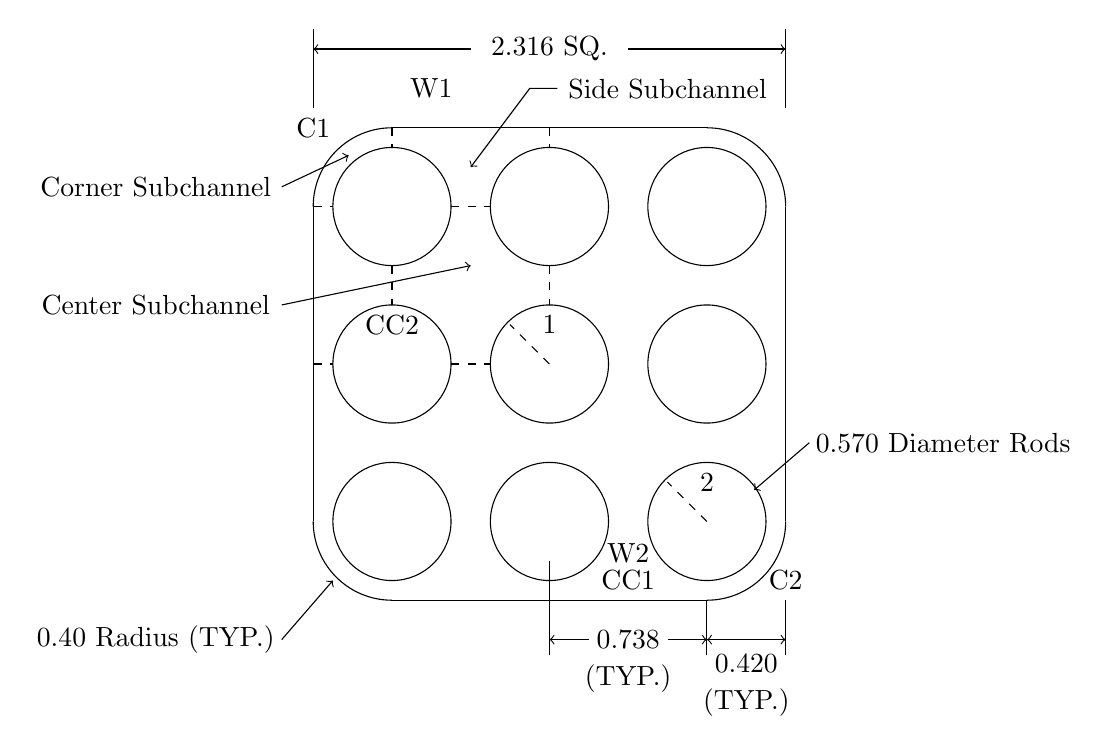
\begin{tikzpicture}

%Rounded corners
\draw (3,2) arc (0:90:1);
\draw (-2,3) arc (90:180:1);
\draw (-3,-2) arc (180:270:1);
\draw (2,-3) arc (270:360:1);

%Grid of circles
\draw (0,0) circle (0.75);
\draw (0,2) circle (0.75);
\draw (0,-2) circle (0.75);
\draw (2,0) circle (0.75);
\draw (2,2) circle (0.75);
\draw (2,-2) circle (0.75);
\draw (-2,0) circle (0.75);
\draw (-2,2) circle (0.75);
\draw (-2,-2) circle (0.75);

%Box
\draw (-3,-2) -- (-3,2);
\draw (3,-2) -- (3,2);
\draw (2,-3) -- (-2,-3);
\draw (-2,3) -- (2,3);

%Misc lines
\draw [dashed] (-2,3) -- (-2,2.75);
\draw [dashed] (0,3) -- (0,2.75);
\draw [dashed] (-2,1.25) -- (-2,0.75);
\draw [dashed] (0,1.25) -- (0,0.75);
\draw [dashed] (-3,2) -- (-2.75,2);
\draw [dashed] (-3,0) -- (-2.75,0);
\draw [dashed] (-1.25,2) -- (-0.75,2);
\draw [dashed] (-1.25,0) -- (-0.75,0);

\draw [dashed] (0,0) -- (-0.5,0.5);
\draw [dashed] (2,-2) -- (1.5,-1.5);

%Misc arrows and labels
\draw [<-] (-3,4) -- (-1,4);
\draw [->] (1,4) -- (3,4);
\draw (-3,4.25) -- (-3,3.25);
\draw (3,4.25) -- (3,3.25);
\draw (0,4) node {2.316 SQ.};

\draw [<-] (0,-3.5) -- (0.5,-3.5);
\draw [->] (1.5,-3.5) -- (2,-3.5);
\draw (2,-3.7) -- (2,-3);
\draw (0,-3.7) -- (0,-2.5);
\draw (1,-3.5) node {0.738};
\draw (1,-4) node {(TYP.)};

\draw [<->] (2,-3.5) -- (3,-3.5);
\draw (3,-3.7) -- (3,-3);
\draw (2.5,-3.8) node {0.420};
\draw (2.5,-4.3) node {(TYP.)};

\draw [->] (-3.4,2.25) -- (-2.55,2.65);
\draw (-5,2.25) node {Corner Subchannel};

\draw [->] (-3.4,0.75) -- (-1,1.25);
\draw (-5,0.75) node {Center Subchannel};

\draw [->] (0.1,3.5) -- (-0.25,3.5) -- (-1,2.5);
\draw (1.5,3.5) node {Side Subchannel};

\draw [->] (-3.4,-3.5) -- (-2.75,-2.75);
\draw (-5,-3.5) node {0.40 Radius (TYP.)};

\draw [->] (3.3,-1) -- (2.6,-1.6);
\draw (5,-1) node {0.570 Diameter Rods};

\draw (-3,3) node {C1};
\draw (-1.5,3.5) node {W1};
\draw (1,-2.75) node {CC1};

\draw (3,-2.75) node {C2};
\draw (1,-2.4) node {W2};
\draw (-2,0.5) node {CC2};

\draw (0,0.5) node {1};
\draw (2,-1.5) node {2};

\end{tikzpicture}
\end{center}
\caption{Position of pressure taps for setting isokinetic conditions. Note splitter positions for the various subchannels.}
\label{fig:position_of_pressure taps}
\caption{Position of Pressure Taps for Setting Isokinetic Conditions \cite{Lahey1970}.}
\label{fig:channel_layout}
\end{figure}

There are nine rods.
There are twenty-four gaps.
It has a high degree of connectivity.

\subsection{Results}
\label{subsect:ge_results}

Here is where I show how the results in great agreement with each other.
Also I will point out the under prediction of the pressure differentials as predicted by \cobra{}.

\section{Simple LWR Quenching Reflood Model}
\label{sect:quench_problem}
This test problem is intended to represent a simplified model of an LWR during the reflood portion of a LOCA.
It was

\subsection{Model}
\label{subsect:quench_model}
The model is as follows:
Here is the geometry:


\subsection{Results}
\label{subsect:quench_results}


